\documentclass[12pt]{article}
\usepackage{amsmath,amssymb,amsthm}
\usepackage{graphicx,mathabx}
\usepackage{xcolor}
\usepackage{tikz}
\usepackage{placeins}
\usepackage{lipsum}
\usepackage[shortlabels]{enumitem}
\begin{document}
\title{TCSS 343 - Week 3}
\author{Jake McKenzie}
\maketitle
\noindent\centerline{\textbf{Master Theorem Practice}}\\\\
\\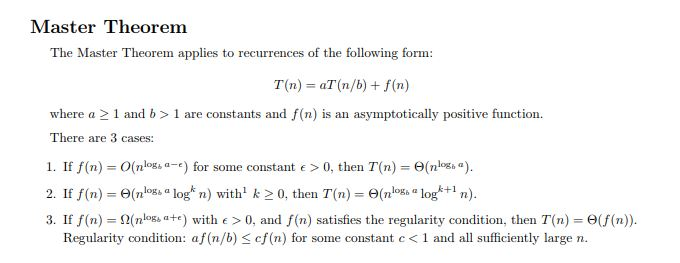
\includegraphics[width=\linewidth]{mt.jpg}\\\\
For the following problems show which case of the master theorem 
each problem goes to. The master theorem is applicable for each 
problem.
\newpage
\noindent 0. \\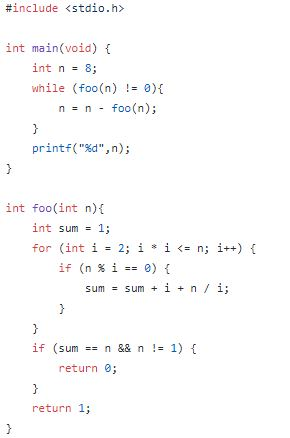
\includegraphics[scale = 1]{debug3_2.jpg}\\
What is the final value of $n$? Use the tracing 
technique we used in last class where you keep 
track of each line.
\newpage
\noindent 1. $T(n)$ $=$ $3T(\frac{n}{2})$ $+$ $n^2$\\\\\\\\\\
2. $T(n)$ $=$ $4T(\frac{n}{2})$ $+$ $n^2\log{n}$\\\\\\\\\\
3. $T(n)$ $=$ $3T(\frac{n}{4})$ $+$ $n\log{n}$\\\\\\\\\\
4. $T(n)$ $=$ $2T(\frac{n}{4})$ $+$ $2$\\\\\\\\\\
5. $T(n)$ $=$ $T(\frac{n}{4})$ $+$ $\log{n}$\\\\\\\\\\
6. $T(n)$ $=$ $2T(\frac{n}{4})$ $+$ $\sqrt{n}$\\\\\\\\\\
7. $T(n)$ $=$ $2T(\frac{n}{4})$ $+$ $n^{0.51}$\\\\\\\\\\
\newpage
\noindent 8. $T(n)$ $=$ $3T(\frac{n}{2})$ $+$ $n$\\\\\\\\\\
9. $T(n)$ $=$ $4T(\frac{n}{2})$ $+$ $n$\\\\\\\\\\
A. $T(n)$ $=$ $3T(\frac{n}{3})$ $+$ $\frac{n}{2}$\\\\\\\\\\
B. $T(n)$ $=$ $4T(\frac{n}{2})$ $+$ $\frac{n}{\log{n}}$\\\\\\\\\\
C. $T(n)$ $=$ $T(\frac{n}{3})$ $+$ $n^2$\\\\\\\\\\
D. $T(n)$ $=$ $8T(\frac{n}{3})$ $+$ $2^n$\\\\\\\\\\
E. $T(n)$ $=$ $16T(\frac{n}{4})$ $+$ $n$\\\\\\\\\\
\newpage
\noindent F. $T(n)$ $=$ $2T(\frac{n}{4})$ $+$ $n!$\\\\\\\\\\
10. $T(n)$ $=$ $0.5T(\frac{n}{2})$ $+$ $\frac{1}{n}$\\\\\\\\\\
11. $T(n)$ $=$ $16T(\frac{n}{4})$ $+$ $n!$\\\\\\\\\\
12. $T(n)$ $=$ $9T(\frac{n}{3})$ $+$ $n^2$\\\\\\\\\\
13. $T(n)$ $=$ $7T(\frac{n}{3})$ $+$ $\cos{n}$\\\\\\\\\\
14. $T(n)$ $=$ $8T(\frac{n}{3})$ $+$ $1$\\\\\\\\\\
15. $T(n)$ $=$ $T(\frac{n}{2})$ $+$ $n^3$\\\\\\\\\\
\end{document}